

\chapter{基于度量学习的神经网络不确定性研究}
\section{引言}

在机器学习和深度学习的研究与应用中,高维特征的分布建模与分析始终是一个核心挑战。对这些高维特征进行概率密度建模,不仅能够有效捕捉数据的分布特征,还能支持异常检测、不确定性量化和生成建模等任务。传统分类方法中,交叉熵损失函数(Cross Entropy Loss)广泛应用于监督学习任务,通过最小化预测类别与真实类别之间的差异来优化模型性能。然而,在高维特征空间中,分类器可能会受到类别间重叠和样本分布稀疏性等问题的影响,这使得直接对概率密度进行建模变得困难。因此,在解决这一问题时,度量学习(Metric Learning)作为一种优化特征空间表示的技术,提供了一种有效的解决思路。

度量学习\cite{kaya2019deep}\cite{kulis2013metric}\cite{yang2566distance}是机器学习中的一个重要分支,旨在学习适用于特定任务的距离度量。该方法通常用于度量特征空间中样本之间的相似度或差异度,广泛应用于人脸识别、图像检索、推荐系统、自然语言处理等领域。度量学习的核心目标是学习一个距离函数,使得相似样本在距离空间中接近,不相似样本远离。与传统的分类或回归任务不同,度量学习通过优化样本之间的相对距离关系,而非直接优化类别预测,从而间接提高任务性能。度量学习中的距离函数通常可以是欧几里得距离、马氏距离、余弦相似度等。根据学习方式的不同,度量学习方法可以分为两类:一类基于距离函数的学习算法,另一类基于相似度/差异度的学习算法。常见的度量学习算法包括Siamese网络\cite{bromley1994signature}、三元组网络\cite{schroff2015facenet}、对比损失\cite{hadsell2566dimensionality}等。

本文提出了一种通过神经网络训练引入度量学习约束的方法,使得高维特征空间的样本分布更加适合高斯混合模型(GMM)进行概率密度建模。特征空间的性质对不确定性的建模效果有着重要影响,而度量学习可以通过优化特征表示,使相似样本更加紧密,不相似样本更远离,从而有效减少高维空间中不确定性建模的复杂性。此外,度量学习有助于提高特征分布的聚集性和可分性,从而提高概率密度估计的精度。本章通过引入辅助损失函数(Auxiliary Loss),结合交叉熵损失函数共同训练(如图\ref{tag:模型结构图2}所示),实现了特征空间的类内紧密性和类间可分性,从而提升了基于高维特征的概率密度建模神经网络不确定性的效果,并在OOD检测等任务上进行了验证。

此外,随着深度学习的广泛应用,特征降维技术已成为高效数据处理和分析的重要工具。由于神经网络提取的高维特征可能维度过高(如ResNet50提取的特征维度为2048维),这可能导致维度灾难\cite{murphy2012machine}、计算复杂度过高以及过拟合等问题。为了有效进行概率密度建模和计算,本章研究了降维技术的应用,提出采用主成分分析(PCA,Principal Component Analysis)作为降维方法,旨在减少GMM在对高维特征建模上参数的存储空间。PCA是一种广泛应用于数据压缩、特征选择和数据可视化等领域的降维技术。本章将PCA用于对高维特征进行降维,并在降维后的特征上重新建立高斯混合模型。通过理论分析PCA降维前后的时间复杂度和空间复杂度,并通过实验验证,高斯混合模型结合PCA降维能够显著减少存储空间需求,并提高建模效率。



\section{主要方法}
\subsection{辅助损失函数联合训练}

首先介绍下高维特征空间上的类内紧密性和类间可分性,如图\ref{interintra}。

\begin{figure}[h]
    \centering
    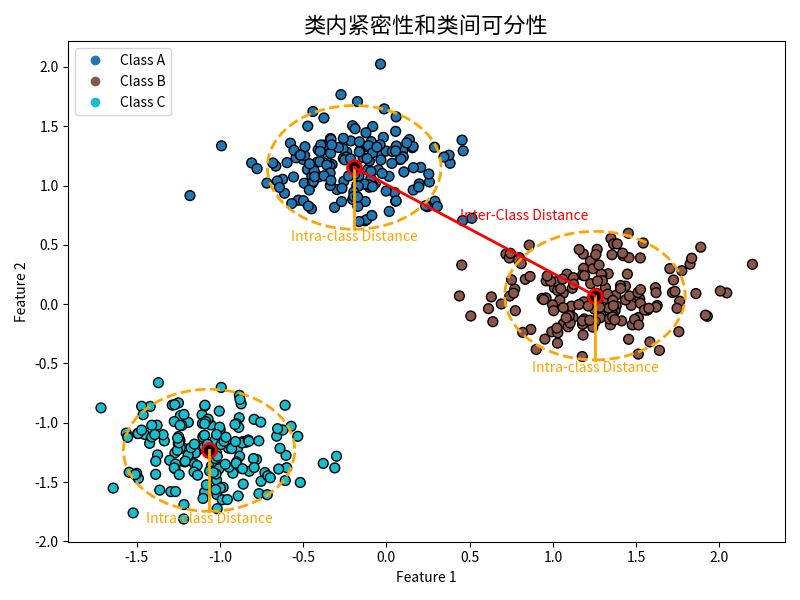
\includegraphics[width=1.\linewidth]{assets/inter-intra.png}
    \caption{类内紧密性和类间可分性}
    \label{interintra}
\end{figure}

类内紧密性(Intra-class Compactness)指的是同一类别的样本在特征空间中分布得多么紧凑,提升类内紧密性的目的是使同一类别的样本在特征空间中更接近。高类内紧密性意味着表示同一类别的样本在特征空间中聚集在一起,样本的特征能够很好地描述同一类别的特性,减少了同一类别样本之间的差异。 类间可分性(Inter-class Separability)指的是不同类别的样本在特征空间中的分离程度,提升类间可分性的目的是使不同类别的样本在特征空间中相距更远。高类间可分性意味着不同类别在特征空间中有更明显的分隔,类别之间有明显的边界,这有助于分类器在决策边界上更好地区分不同类别。理想状态下,在特征空间中,同一类别的样本应该分布紧密(即高类内紧密性),而不同类别的样本之间应该相距较远(即高类间可分性)。但是当数据维度增加或样本类别分布复杂时,这两者可能会受到限制。例如,噪声数据会降低类内紧密性,而类别间的相似性会降低类间可分性。通过优化类内紧密性和类间可分性,分类模型能够更高效地学习特征表示,提高分类的准确性。



CenterLoss\cite{wen2016discriminative}是一种用于深度学习中的损失函数,主要应用于人脸识别和特征嵌入学习等任务。其核心目标是通过最小化同一类别样本特征向量与该类中心之间的欧几里得距离,优化特征空间中的类内距离,从而提高模型的区分能力。具体而言,CenterLoss 强调使同类样本在特征空间中更加紧凑,减少类别间的重叠,并保持不同类别样本之间较大的距离。其原始形式定义为:

\[
L_{\text{center}} = \frac{1}{2N} \sum_{i=1}^{N} \| f(x_i) - c_{y_i} \|^2
\]

其中,\( f(x_i) \) 表示输入样本 \( x_i \) 的特征表示,\( c_{y_i} \) 为类别 \( y_i \) 的类别中心,\(\|\cdot\|\) 是欧几里得距离,\( N \) 为样本数量。通过这种方式,CenterLoss 使得同类别的样本在特征空间中更加集中,从而提升分类性能和类别区分能力。在实际应用中,CenterLoss 通常与 Softmax 损失函数结合使用,进一步增强模型的分类效果。组合损失函数的表达式为:

\[
L = L_{\text{softmax}} + \lambda * L_{\text{center}}
\]

其中,\(L_{\text{softmax}}\) 是传统的分类损失,目标是最小化类别预测误差,\(\lambda\) 是超参数,调节 CenterLoss 和 Softmax 损失之间的权重平衡。通过联合优化这两个损失,网络不仅能够学习到更精确的分类决策,还能够使得特征空间中的样本更加紧凑和可区分。



% \begin{figure}[h]
%     \centering
%     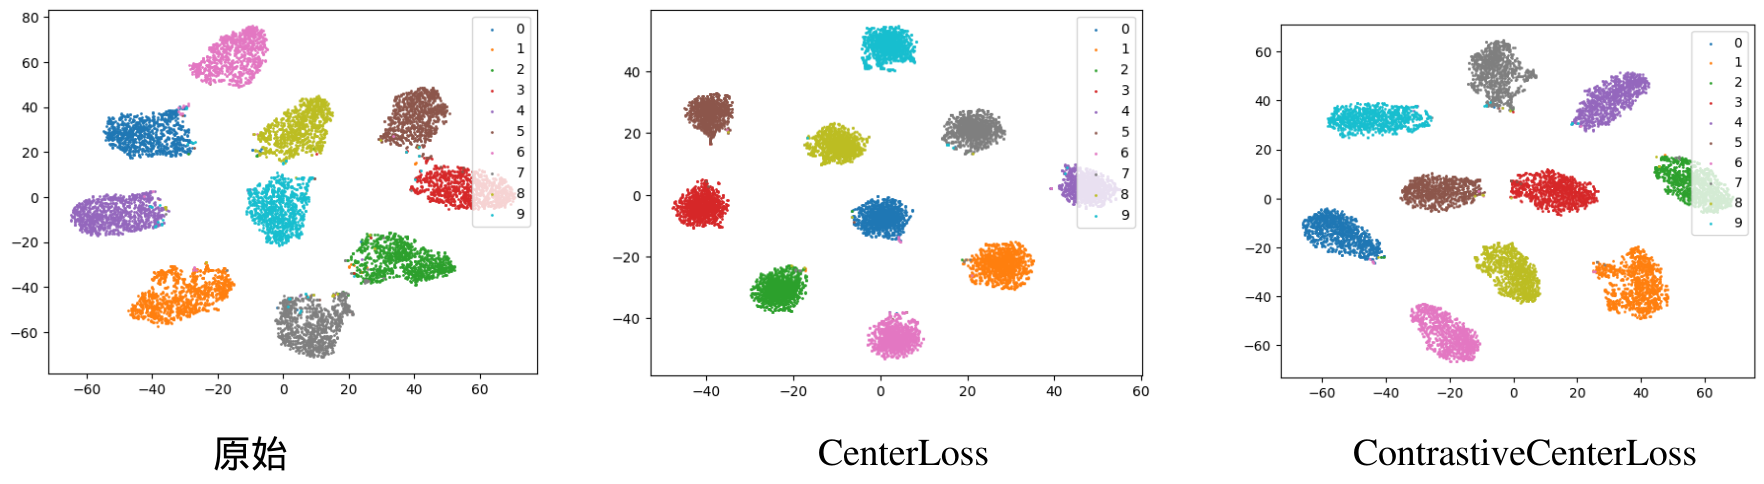
\includegraphics[width=1.\linewidth]{assets/4-1.png}
%     \caption{MNIST+VGG16,特征空间上的t-SNE可视化}
%     \label{fig:MNIST-t-SNEl}
% \end{figure}
% 本文首先在MNIST数据集上训练了一个分类网络VGG16,分别使用CrossEntropyLoss单独训练和CrossEntropyLoss与CenterLoss联合训练的方式。实验结果如图\ref{fig:MNIST-t-SNEl}。

% 观察图\ref{fig:MNIST-t-SNEl},在没有 CenterLoss 的情况下,同一类的样本可能会在特征空间中分布较散,类别间可能会有重叠。在加入 CenterLoss 后,同类样本会更加集中,类别间的重叠减少,类与类之间的距离增大。同时注意到,加入CenterLoss后类内紧密性变好,但是类间可分性变差了。


从CenterLoss的定义上看,仅仅包含类内紧密性的损失函数,为了提高特征空间上的类间可分性,可以考虑在其原始公式的分母上引入一些提高类间可分性的项。这种改进可以通过设计一个新的权重项,使得在计算类间距离时,能够更强调类别间的分隔性,从而增强不同类别特征的区分度。为了提高类间可分性,可以对原公式做一些改进。一个简单的策略是加入与类别间距离相关的项,从而惩罚相近类别的样本特征,使得类别之间的边界更加清晰。可以通过将分母中加入一个与类别中心间距相关的因子来增强类间可分性,具体如下:

\[
\text{AuxLoss} = \frac{1}{2} \sum_{i=1}^m \frac{\|x_i - C_{y_i}\|_2^2}{\sum_{j=1, j \neq y_i}^{m} \|C_{y_i} - C_j\|_2^2 + \delta}.
\],

这里 \( C \) 是类别数,\( c_k \) 是类别 \( k \) 的中心,\( \delta \) 是一个小常数,用于数值稳定性,防止除零错误。

通过在分母中引入$\sum_{j=1, j \neq y_i}^{m} \|C_{y_i} - C_j\|_2^2$,让距离较远的类别中心在优化过程中贡献更少的惩罚项,反之,距离较近的类别中心将会对损失值产生更大的影响。这种方式鼓励类别间的分隔,使得样本的特征在同一类别内紧凑、而在不同类别间具有更大的间隔。随着训练的进行,样本在特征空间中的分布会越来越偏向于形成更加清晰的类别分隔。通过调整类别间距的方式,可以有效减少类间重叠,从而增强模型对不同类别的区分能力。

这种改进后的AuxLoss可以作为辅助损失加入到交叉熵损失函数中(如图\ref{tag:模型结构图2},进一步强化特征的聚合与类间分隔。在训练过程中,原本的交叉熵损失负责指导分类准确性,而改进后的AuxLoss则帮助网络在优化特征表示时,通过引入类别中心之间的间距来进一步优化类别分离的效果,更好地考虑到类别之间的相对距离。

% \begin{figure}[h]
%     \centering
%     \begin{tikzpicture}[
%         node distance=1.5cm and 1.5cm,
%         every node/.style={minimum height=1.2cm, text width=2.0cm, align=center},
%         feature/.style={fill=blue!20},
%         gmm/.style={fill=orange!50,text width={1.0cm}},
%         fc/.style={fill=orange!50,text width={1.0cm}},
%         softmax/.style={fill=orange!50},
%         PCA/.style={fill=red!50},
%         output/.style={fill=gray!30},
%         arrow/.style={-{Stealth[scale=1.2]}},
%         backward/.style={dashed, red, thick} % 红色虚线样式
%     ]
%     % Nodes
%     \node (image) {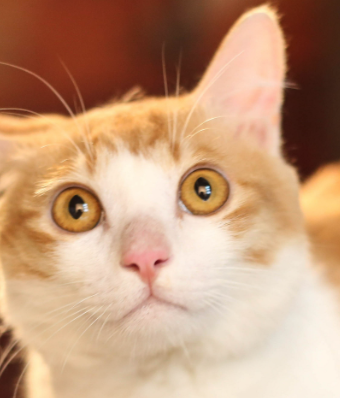
\includegraphics[width=1.5cm]{assets/cat.png}};
%     \node[below=0.2cm of image, align=center] (input_label) {输入$x$};
%     \node[feature, right=of image, trapezium, trapezium angle=60, fill=blue!20, minimum width=1.8cm, minimum height=1.5cm, shape border rotate=270] (feature_extractor) {feature extractor};
%     \node[below=0.2cm of feature_extractor, align=center] (input_label) {$f_\theta$};
    
%     % 条形图节点
%     \node[right=1cm of feature_extractor, inner sep=0] (bar_chart) {
%         \begin{tikzpicture}[scale=0.9]
%             % 绘制主条
%             \draw[thick] (0,0) rectangle (0.5,5); % 外框
%             % 分块填充
%             \fill[black!80] (0,4.5) rectangle (0.5,5);
%             \fill[gray!10] (0,4.0) rectangle (0.5,4.5);
%             \fill[gray!50] (0,3.5) rectangle (0.5,4);
%             \fill[black!70] (0,3) rectangle (0.5,3.5);
%             \fill[gray!70] (0,2.5) rectangle (0.5,3);
%             \fill[gray!20] (0,2) rectangle (0.5,2.5);
%             \fill[black!40] (0,1.5) rectangle (0.5,2);
%             \fill[gray!30] (0,1) rectangle (0.5,1.5);
%             \fill[black!80] (0,0.5) rectangle (0.5,1);
%             \fill[gray!60] (0,0) rectangle (0.5,0.5);
%         \end{tikzpicture}
%     };
%     \node[below=0.2cm of bar_chart, align=center] (input_label) {$z$};

%     % \node[PCA, right=of bar_chart] (PCA) {PCA};
%     % 其他节点
%     \node[output, above right=0.001cm and 0.5cm of bar_chart] (gmm) {AuxLoss};
%     % \node[below=0.1cm of gmm, align=center] (input_label) {$q(z)$};
%     \node[fc, below right=0.001cm and 0.5cm of bar_chart] (fc) {FC};
%     % \node[softmax, right=1.0cm of fc] (softmax) {Softmax};
%     \node[output, right=1.0cm of fc] (probs) {CELoss};
%     % \node[below=0.1cm of probs, align=center] (input_label) {$p(x)$};
%     % \node[output, right=1.0cm of gmm] (logPx) {Uncertainty};
%     % \node[below=0.1cm of logPx, align=center] (input_label) {$\log q(z)$};
    
%     % Paths
%     \draw[arrow] (image) -- (feature_extractor);
%     \draw[arrow] (feature_extractor) -- (bar_chart);
%     % \draw[arrow] (bar_chart) -- (PCA);
%     \draw[arrow] (bar_chart) -- (gmm);
%     \draw[arrow] (bar_chart) -- (fc);
%     % \draw[arrow] (gmm) -- (logPx);
%     % \draw[arrow] (fc) -- (softmax);  
%     \draw[arrow] (fc) -- (probs);


%     \end{tikzpicture}
%     \caption{基于高维特征概率密度建模的模型不确定性}
%     \label{tag:模型结构图2}
% \end{figure}


\begin{figure}[h]
    \centering
    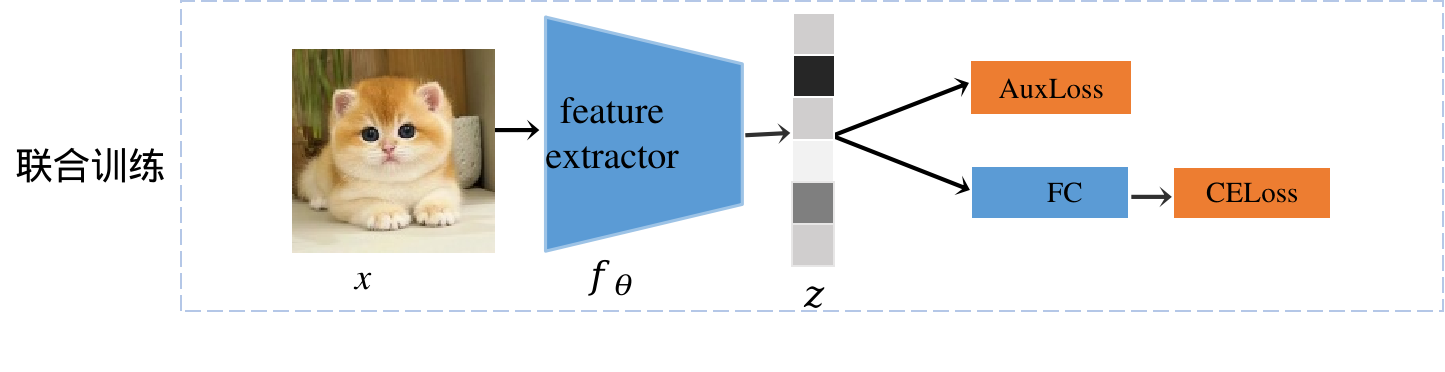
\includegraphics[width=1.\linewidth]{assets/structure2.png}
    \caption{基于高维特征概率密度建模的模型不确定性}
    \label{tag:模型结构图2}
\end{figure}


CrossEntropyLoss和AuxLoss联合训练的公式如下:
\begin{equation}
    L = L_s+\lambda * L_x
\end{equation}

其中,$L_s$是CrossEntropyLoss,公式如下:

\begin{equation}
    L_s= - \sum_{i=1}^C y_i \log\left(\frac{\exp(z_i)}{\sum_{j=1}^C \exp(z_j)}\right)
\end{equation}

$L_x$是修正后的AuxLoss,公式如下:
\begin{equation}
    L_x = \frac{1}{2}\sum_{i=1}^{m} \frac{\Vert x_i-C_{y_i}\Vert_2^2}{\sum_{j=1,j\neq y_i}^{m}\Vert C_i-C_j\Vert_2^2+\delta}
\end{equation}

上述AuxLoss,分子项通过特征向量与其对应类别中心距离的最小化保证类内紧密性,分母项通过不同类别中心的距离最大化来保证类间可分性。在具体实现时,类别中心是基于正态分布随机初始化的,它会作为模型的一部分进行学习和优化。类别中心会随着模型的训练过程而更新,类别中心作为模型参数的一部分,损失函数反向传播时,PyTorch框架通过优化器自动更新类别中心的值。关于上述AuxLoss的损失函数求导,有以下的结论。

\textbf{性质4.1:}
给定的损失函数如下:

\[
L_x = \frac{1}{2} \sum_{i=1}^m \frac{\|x_i - C_{y_i}\|_2^2}{\sum_{j=1, j \neq y_i}^{m} \|C_{y_i} - C_j\|_2^2 + \delta}.
\]
其中:
\( x_i \) 是第 \( i \) 个样本的输入,\( y_i \) 是第 \( i \) 个样本的类别标签,\( C_k \) 是类别 \( k \) 的特征中心,\( \delta \) 是一个正的平滑常数。则关于每个类中心的梯度为:


当 \( j = y_i \) 时:
\[
\frac{\partial L_x}{\partial C_j} =  \sum_{i: y_i = j} \left( \frac{- (x_i - C_j)}{B_i} - \frac{A_i}{B_i^2} \sum_{k=1, k \neq j}^m  (C_j - C_k) \right).
\]

当 \( j \neq y_i \) 时:
\[
\frac{\partial L_x}{\partial C_j} = -\sum_{i: y_i \neq j} \left( \frac{A_i}{B_i^2} (C_{y_i} - C_j) \right).
\]


\textbf{证明}:
需要对损失函数求关于 \( C_j \) 的梯度。为了方便,将损失函数记为:

\[
L_x = \frac{1}{2} \sum_{i=1}^m \frac{A_i}{B_i},
\]

其中:
\[
A_i = \|x_i - C_{y_i}\|_2^2, \quad B_i = \sum_{j=1, j \neq y_i}^m \|C_{y_i} - C_j\|_2^2 + \delta.
\]

\[
\frac{\partial L_x}{\partial C_j} = \frac{1}{2} \sum_{i=1}^m \frac{\partial}{\partial C_j} \left( \frac{A_i}{B_i} \right).
\]

使用商的求导法则:
\[
\frac{\partial}{\partial C_j} \left( \frac{A_i}{B_i} \right) = \frac{1}{B_i} \frac{\partial A_i}{\partial C_j} - \frac{A_i}{B_i^2} \frac{\partial B_i}{\partial C_j}.
\]

因此,梯度可以分解为两部分:
\[
\frac{\partial L_x}{\partial C_j} = \frac{1}{2} \sum_{i=1}^m \left( \frac{1}{B_i} \frac{\partial A_i}{\partial C_j} - \frac{A_i}{B_i^2} \frac{\partial B_i}{\partial C_j} \right).
\]

1.求 \( \frac{\partial A_i}{\partial C_j} \):

当 \( j = y_i \) 时:
\[
A_i = \|x_i - C_{y_i}\|_2^2, \quad \frac{\partial A_i}{\partial C_j} = \frac{\partial}{\partial C_j} \|x_i - C_j\|_2^2 = -2 (x_i - C_j).
\]

当 \( j \neq y_i \) 时:
\[
A_i \text{ 与 } C_j \text{ 无关,因此 } \frac{\partial A_i}{\partial C_j} = 0.
\]

2.求 \( \frac{\partial B_i}{\partial C_j} \)
\[
B_i = \sum_{k=1, k \neq y_i}^m \|C_{y_i} - C_k\|_2^2 + \delta.
\]

当 \( j = y_i \) 时:
\[
\frac{\partial B_i}{\partial C_j} = \frac{\partial}{\partial C_j} \sum_{k=1, k \neq y_i}^m \|C_j - C_k\|_2^2 = \sum_{k=1, k \neq y_i}^m 2 (C_j - C_k).
\]

当 \( j \neq y_i \) 时:
\[
\frac{\partial B_i}{\partial C_j} = \frac{\partial}{\partial C_j} \|C_{y_i} - C_j\|_2^2 = -2 (C_{y_i} - C_j).
\]


综合梯度,将以上结果代入:

当 \( j = y_i \) 时:
\[
\frac{\partial L_x}{\partial C_j} =  \sum_{i: y_i = j} \left( \frac{- (x_i - C_j)}{B_i} - \frac{A_i}{B_i^2} \sum_{k=1, k \neq j}^m  (C_j - C_k) \right).
\]

当 \( j \neq y_i \) 时:
\[
\frac{\partial L_x}{\partial C_j} = -\sum_{i: y_i \neq j} \left( \frac{A_i}{B_i^2} (C_{y_i} - C_j) \right).
\]


在CIFAR10数据集上训练ResNet50网络,分别使用原始交叉熵损失函数训练网络和使用交叉熵损失函数加辅助损失函数联合训练的方法,训练得到的高维特征难以直接进行可视化分析,所以本文使用t-SNE(t-Distributed Stochastic Neighbor Embedding)\cite{van2568visualizing}方法先对高维特征进行降维到2维空间上。t-SNE是一种常用的降维方法,能够将高维数据映射到二维或三维空间中,同时保持样本间的相对距离。通过在降维后的特征空间中可视化数据点,可以直观地看到类内样本的聚集情况和类别间的分离情况。
t-SNE可视化高维特征空间结果如图\ref{cifar10-tsne}。

\begin{table}[H]
\captionsetup{font=small, justification=centering} % 设置标题字体大小与对齐方式
\centering
\begin{tabular}{|c|c|c|}
\hline
\textbf{} & \textbf{CELoss} & \textbf{CELoss+AuxLoss} \\ \hline % 使表头加粗
\begin{minipage}{0.1\textwidth} \centering VGG \end{minipage} & 
\begin{minipage}{0.45\textwidth} \centering 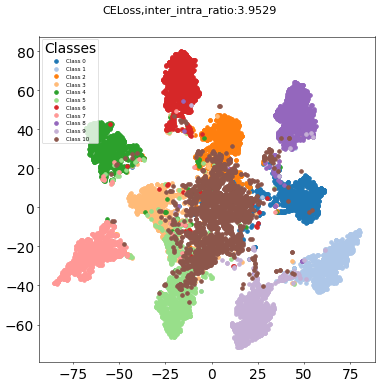
\includegraphics[width=\textwidth]{assets/vgg16_tsne_feature.png} \end{minipage} & 
\begin{minipage}{0.45\textwidth} \centering 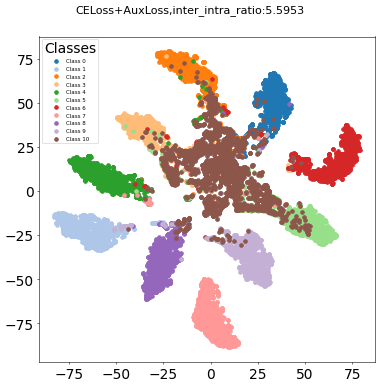
\includegraphics[width=\textwidth]{assets/vgg16_tsne_feature_c.png} \end{minipage} \\ \hline
\begin{minipage}{0.1\textwidth} \centering ResNet \end{minipage} & 
\begin{minipage}{0.45\textwidth} \centering 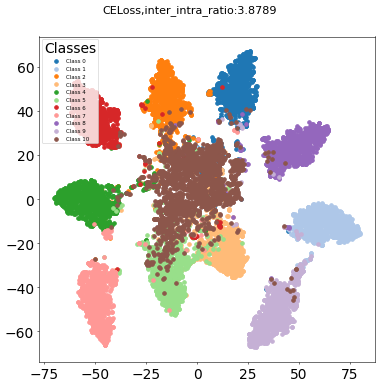
\includegraphics[width=\textwidth]{assets/resnet50_tsne_feature.png} \end{minipage} & 
\begin{minipage}{0.45\textwidth} \centering 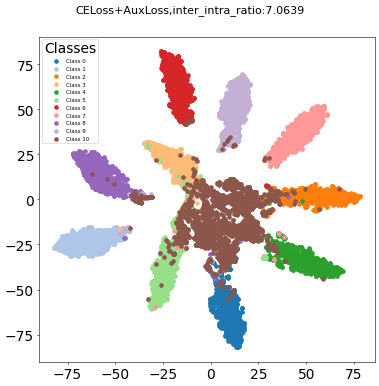
\includegraphics[width=\textwidth]{assets/resnet50_tsne_feature_c.png} \end{minipage} \\ \hline
\begin{minipage}{0.1\textwidth} \centering ViT \end{minipage} & 
\begin{minipage}{0.45\textwidth} \centering 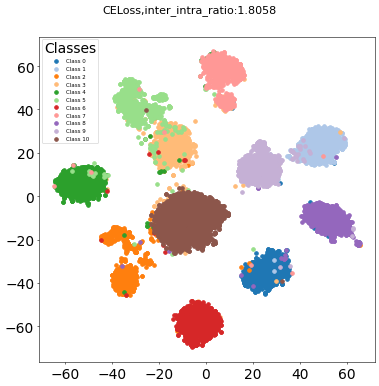
\includegraphics[width=\textwidth]{assets/vit_tsne_feature.png} \end{minipage} & 
\begin{minipage}{0.45\textwidth} \centering 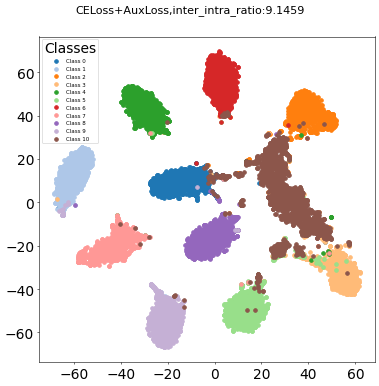
\includegraphics[width=\textwidth]{assets/vit_tsne_feature_c.png} \end{minipage} \\ \hline
\end{tabular}
\caption{CIFAR10数据集,特征空间的t-SNE可视化,左侧为交叉熵损失函数训练,右侧为交叉熵损失函数与辅助损失函数联合训练。}
\label{cifar10-tsne}
\end{table}


左图展示了仅使用交叉熵损失函数训练的结果。从图中可以看出,不同类别的数据点(用不同颜色表示)在特征空间中有一定的分离,但仍然存在一些重叠和模糊的区域。这表明模型在某些类别上的区分能力有限。右图展示了使用交叉熵损失函数和辅助损失函数联合训练的结果。从图中可以看出,不同类别的数据点在特征空间中的分离更加明显,重叠和模糊的区域大大减少。这表明模型在区分不同类别时的能力得到了显著提升。



在本实验中,辅助损失函数的加入使得模型在特征空间中的表示更加清晰和分离,从而提高了分类的准确性。通过对比加辅助损失函数前后的高维特征t-SNE可视化结果,可以明显看出辅助损失函数对模型性能的提升作用。辅助损失函数能提高模型在特征空间中的区分能力,从而提升分类性能,并更容易在高维特征空间上进行概率分布建模。

% \begin{figure}[h]
% \captionsetup{font=small, justification=centering}
%     \centering
%     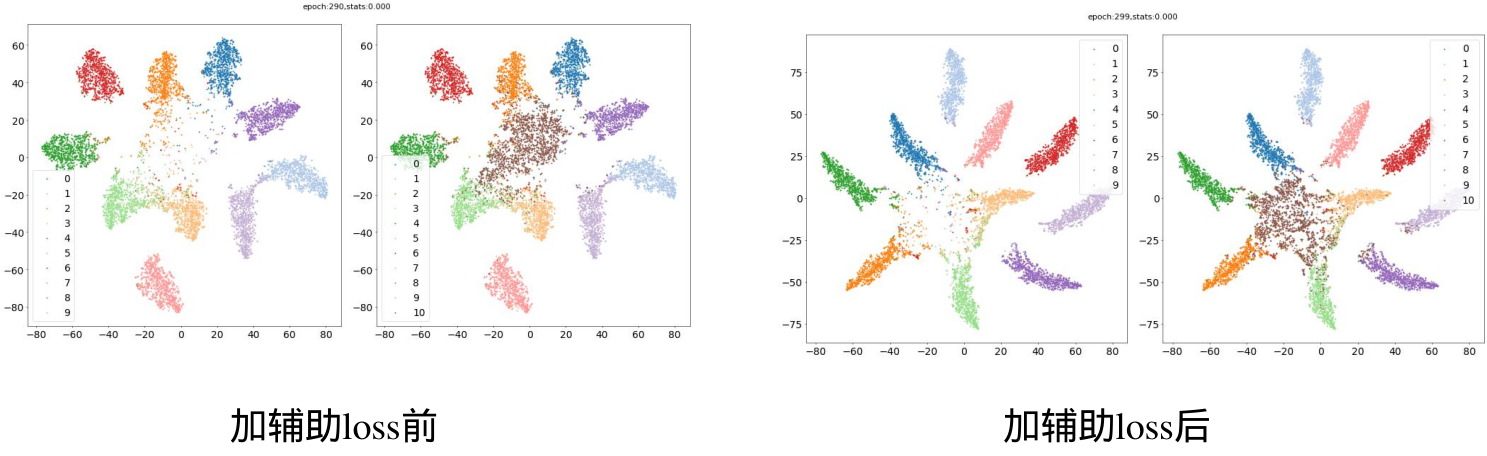
\includegraphics[width=1\linewidth]{assets/4-2.png}
%     \caption{ResNet50+CIFAR10,特征空间的t-SNE可视化,维度D=2048,左边使用交叉熵损失函数训练,右边使用交叉熵损失函数和辅助损失函数联合训练的方法}
%     \label{cifar10-tsne}
% \end{figure}

% \begin{table}[h]
% \captionsetup{font=small, justification=centering}
% \centering
% \begin{tabular}{|c|c|c|}
% \hline
% 模型 & CELOSS & CELOSS+AUXLOSS \\ \hline
% VGG & \includegraphics[width=0.4\textwidth]{assets/vgg_stats_295.jpg} & 
% \includegraphics[width=0.4\textwidth]{assets/vgg_stats_295_c.jpg} \\ \hline
% ResNet & \includegraphics[width=0.4\textwidth]{assets/resnet_stats_295.jpg} & 
% \includegraphics[width=0.4\textwidth]{assets/resnet_stats_298_c.jpg} \\ \hline
% ViT & \includegraphics[width=0.4\textwidth]{assets/vit_stats_297.jpg} & 
% \includegraphics[width=0.4\textwidth]{assets/vit_stats_295_c.jpg} \\ \hline
% \end{tabular}
% \caption{CIFAR10, 特征空间的t-SNE可视化, 维度D=2048,左边使用交叉熵损失函数训练,右边使用交叉熵损失函数和辅助损失函数联合训练的方法}
% \label{cifar10-tsne}
% \end{table}




% \begin{table}[H]
% \captionsetup{font=small, justification=centering} % 设置标题字体大小与对齐方式
% \centering
% \begin{tabular}{|c|c|c|}
% \hline
% \textbf{模型} & \textbf{CELoss} & \textbf{CELoss+AuxLoss} \\ \hline % 使表头加粗
%  VGG &  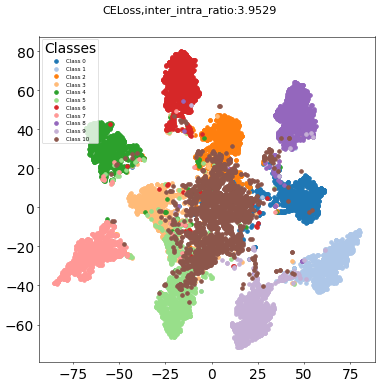
\includegraphics[width=0.4\textwidth]{assets/vgg16_tsne_feature.png} & 
% 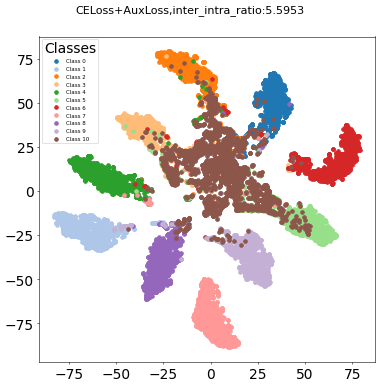
\includegraphics[width=0.4\textwidth]{assets/vgg16_tsne_feature_c.png} \\ \hline
% ResNet & 
%  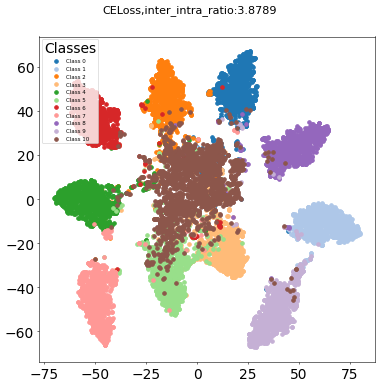
\includegraphics[width=0.4\textwidth]{assets/resnet50_tsne_feature.png} & 
%  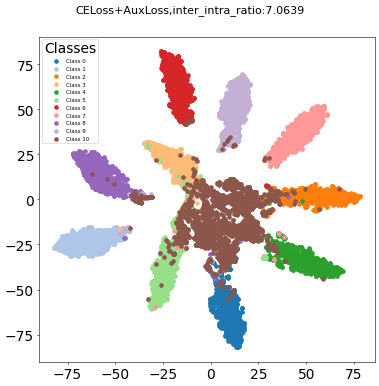
\includegraphics[width=0.4\textwidth]{assets/resnet50_tsne_feature_c.png} \\ \hline
% ViT & 
%  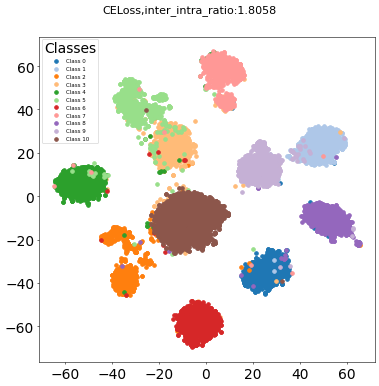
\includegraphics[width=0.4\textwidth]{assets/vit_tsne_feature.png} & 
%  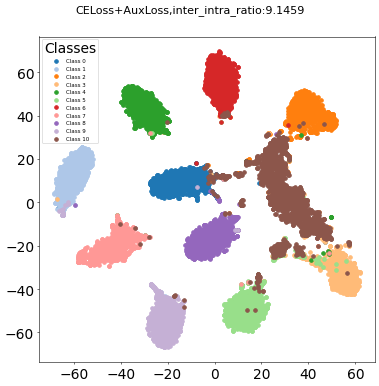
\includegraphics[width=0.4\textwidth]{assets/vit_tsne_feature_c.png} \\ \hline
% \end{tabular}
% \caption{CIFAR10数据集,特征空间的t-SNE可视化,左侧为交叉熵损失函数训练,右侧为交叉熵损失函数与辅助损失函数联合训练。}
% \label{cifar10-tsne}
% \end{table}



为了定量地分析加入辅助损失函数联合训练后,特征空间上类内紧密性和类间可分性的性质,本章使用类内距离、Davies-Bouldin 指数 (DBI)、类间距离、Fisher 比率 (F值) 和 轮廓系数 (Silhouette Coefficient)等几个指标度量,在测试集上计算这几个指标,结果见表\ref{feature_analysis}。以下是关于 类内距离、Davies-Bouldin 指数 (DBI)、类间距离、Fisher 比率 (F值) 和 轮廓系数 (Silhouette Coefficient) 的详细介绍及公式。

类内距离 (Intra-class Distances)衡量同一类别中所有样本对之间的平均距离,反映同一类样本的紧密程度。
\[
D_{\text{intra}}(C_k) = \frac{1}{|C_k|^2} \sum_{i \in C_k} \sum_{j \in C_k} d(x_i, x_j)
\]
其中:$C_k$是类 $k$ 中的样本集合, $|C_k|$是类 $k$ 的样本数量 $d(x_i, x_j)$是样本 $x_i$ 和 $x_j$ 之间的距离。

类间距离 (Inter-class Distances)用于衡量不同聚类之间的分离程度,通常计算聚类中心之间的距离。

\[
D_{inter} = \sum_{i=1}^{C} N_i (\mu_i - \mu)^2
\]

其中:  \( C \) 是类别的数量,   \( N_i \) 是第 \( i \) 类的样本数量,  \( \mu_i \) 是第 \( i \) 类的均值, \( \mu \) 是所有样本的全局均值。该公式表示各个类别均值 \( \mu_i \) 与全局均值 \( \mu \) 之间的加权距离,权重为各类别的样本数量 \( N_i \)。

Davies-Bouldin 指数 (DBI)衡量聚类的质量,综合考虑了类内紧密性和类间分离性,值越小表示聚类效果越好。
\[
DBI = \frac{1}{K} \sum_{k=1}^K \max_{j \neq k} \frac{S_k + S_j}{d_{kj}}
\]
其中:$K$是类别数;$S_k$是类 $k$ 的类内散布性(如类内平均距离);$d_{kj}$是聚类 $k$ 和聚类 $j$ 的中心之间的距离。




Fisher Ratio(费舍尔比率)用于衡量不同类别之间的可分性,通常定义为类间散布和类内散布的比值。其公式为:

\[
F = \frac{S_B}{S_W}
\]

其中, \( S_B \) 表示类间散布(between-class scatter),  \( S_W \) 表示类内散布(within-class scatter)。
类间散布 \( S_B \) 定义为:$S_B = \sum_{i=1}^C N_i (\mu_i - \mu)^2$,其中:  \( C \) 是类别数量,   \( N_i \) 是第 \( i \) 类的样本数量,   \( \mu_i \) 是第 \( i \) 类样本的均值,  \( \mu \) 是所有样本的全局均值。类内散布 \( S_W \) 定义为:$S_W = \sum_{i=1}^C \sum_{x \in \mathcal{D}_i} (x - \mu_i)^2 $
其中:  \( \mathcal{D}_i \) 是第 \( i \) 类的样本集合,  \( x \) 是样本点。当 \( S_B \) 较大、\( S_W \) 较小时,Fisher Ratio 趋向较大值,表示特征具有较强的区分能力。  当 \( S_B \) 和 \( S_W \) 相近时,Fisher Ratio 较小,表示该特征对类别区分的贡献较弱。


轮廓系数 (Silhouette Coefficient)用于评估聚类的紧密性和分离性,取值范围为 $[-1, 1]$。值越接近 $1$ 表示聚类效果越好。单个样本 $i$ 的轮廓系数定义为:
\[
s(i) = \frac{b(i) - a(i)}{\max(a(i), b(i))}
\]

其中:$a(i)$是样本 $i$ 到其所在聚类中其他样本的平均距离(类内距离);$b(i)$是样本 $i$ 到最邻近的其他聚类的所有样本的平均距离(类间距离)。总体轮廓系数为所有样本轮廓系数的平均值:
\[
S = \frac{1}{N} \sum_{i=1}^N s(i)
\]


\begin{table}[h]
\captionsetup{font=small, justification=centering}
\centering
\renewcommand{\arraystretch}{1.2} % 调整行间距
\setlength{\tabcolsep}{6pt} % 调整列间距
\resizebox{\textwidth}{!}{ % 缩放表格以适应页面宽度
\begin{tabular}{c c c c c c c}
\hline
\textbf{训练策略} & \textbf{Model} & \textbf{IntraClassDistance($\downarrow$)} & \textbf{DaviesBouldinIndexs($\downarrow$)} & \textbf{InterClassDistances($\uparrow$)} & \textbf{FisherRatios($\uparrow$)} & \textbf{SilhouetteCoefficients($\uparrow$)} \\ 
\hline
\multirow{3}{*}{CE Loss} 
& VGG16 & 1.8466 & 0.3687   & 11.4856 & 13.3970 & 0.7520 \\ 
& ResNet50 & \textbf{1.5544}  & 0.3775  & 9.4415 & 13.8453 & 0.7408 \\ 
& VIT & 5.6329 & 0.8430 & 14.7451 & 3.6832 & 0.5080 \\ 
\hline
\multirow{3}{*}{联合训练} 
& VGG16 & \textbf{0.7806}  & \textbf{0.0981} & \textbf{19.4277} & \textbf{136.1505} & \textbf{0.9360} \\ 
& ResNet50 & 3.0138  & \textbf{0.1952} & \textbf{34.6706} & \textbf{44.3006} & \textbf{0.8675} \\ 
& VIT & \textbf{2.3761} & \textbf{0.1937} & \textbf{30.1605} & \textbf{89.0348} & \textbf{0.8698} \\ 
\hline
\end{tabular}
}
\caption{对比加入辅助损失函数前后特征空间类内紧密性和类间可分性的变化}
\label{feature_analysis}
\end{table}

在实验结果中,加入辅助损失函数后,所有模型在特征空间中的类内紧密性和类间可分性均有显著提升。从类内距离和Davies-Bouldin指数(DBI)来看,联合训练的模型相比于仅使用交叉熵损失(CE Loss)能够显著降低类内样本之间的距离,同时DBI指数也得到了明显改善,这表明类内的紧密性得到了增强。类间距离和Fisher比率则呈现出明显的上升,表明类别之间的间隔增大,模型对不同类别的区分度得到了增强。轮廓系数也有所提高,进一步验证了样本在特征空间中的分离效果。

综上所述,加入辅助损失函数能够有效提高模型在特征空间中的类内紧密性和类间可分性。这一改进不仅优化了样本的聚合效果,还增强了类别之间的分隔性,进而提高了模型在分类任务中的表现。


\subsection{PCA降维}

高维特征概率密度建模旨在对高维数据的分布进行概率密度估计,通常用于描述样本的分布特征。随着数据维度的增加,数据的分布往往变得稀疏,如何有效地建模这种稀疏性,成为高维数据分析中的重要挑战。高维数据带来的主要问题包括维度灾难、计算复杂度和过拟合风险。首先,随着特征维度的增加,数据点之间的距离逐渐增大,导致数据变得稀疏。在高维空间中,距离度量(如欧氏距离)逐渐失效,使得有效的概率密度建模变得更加困难。其次,随着维度的增加,计算复杂度急剧上升,尤其是对于基于密度估计的非参数方法(如核密度估计),需要大量计算资源,并且容易受到噪声的干扰。最后,高维数据的稀疏性使得模型容易过拟合训练数据,捕捉到噪声而非数据的真实结构,从而导致模型泛化能力下降。为了解决高维数据存在的上述问题,主要的思路是使用机器学习中的降维技术。

% \begin{figure}[h]
%     \centering
%     \begin{tikzpicture}[
%         node distance=1.5cm and 1.5cm,
%         every node/.style={minimum height=1.2cm, text width=2.0cm, align=center},
%         feature/.style={fill=blue!20},
%         gmm/.style={fill=orange!50,text width={1.0cm}},
%         fc/.style={fill=orange!50,text width={1.0cm}},
%         softmax/.style={fill=orange!50},
%         PCA/.style={fill=red!50},
%         output/.style={fill=gray!30},
%         arrow/.style={-{Stealth[scale=1.2]}},
%         backward/.style={dashed, red, thick} % 红色虚线样式
%     ]
%     % Nodes
%     \node (image) {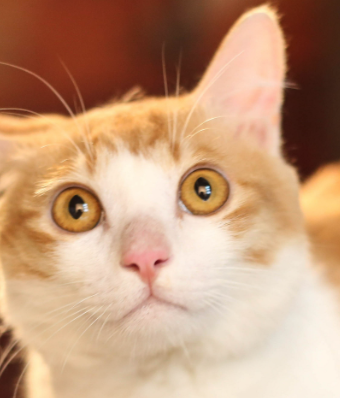
\includegraphics[width=1.5cm]{assets/cat.png}};
%     \node[below=0.2cm of image, align=center] (input_label) {输入$x$};
%     \node[feature, right=of image, trapezium, trapezium angle=60, fill=blue!20, minimum width=1.8cm, minimum height=1.5cm, shape border rotate=270] (feature_extractor) {feature extractor};
%     \node[below=0.2cm of feature_extractor, align=center] (input_label) {$f_\theta$};
    
%     % 条形图节点
%     \node[right=1cm of feature_extractor, inner sep=0] (bar_chart) {
%         \begin{tikzpicture}[scale=0.9]
%             % 绘制主条
%             \draw[thick] (0,0) rectangle (0.5,5); % 外框
%             % 分块填充
%             \fill[black!80] (0,4.5) rectangle (0.5,5);
%             \fill[gray!10] (0,4.0) rectangle (0.5,4.5);
%             \fill[gray!50] (0,3.5) rectangle (0.5,4);
%             \fill[black!70] (0,3) rectangle (0.5,3.5);
%             \fill[gray!70] (0,2.5) rectangle (0.5,3);
%             \fill[gray!20] (0,2) rectangle (0.5,2.5);
%             \fill[black!40] (0,1.5) rectangle (0.5,2);
%             \fill[gray!30] (0,1) rectangle (0.5,1.5);
%             \fill[black!80] (0,0.5) rectangle (0.5,1);
%             \fill[gray!60] (0,0) rectangle (0.5,0.5);
%         \end{tikzpicture}
%     };
%     \node[below=0.2cm of bar_chart, align=center] (input_label) {$z$};

%     \node[PCA, right=of bar_chart] (PCA) {PCA};
%     % 其他节点
%     % \node[output, above right=0.001cm and 0.5cm of bar_chart] (gmm) {AuxLoss};
%     % \node[below=0.1cm of gmm, align=center] (input_label) {$q(z)$};
%     % \node[fc, below right=0.001cm and 0.5cm of bar_chart] (fc) {FC};
%     % \node[softmax, right=1.0cm of fc] (softmax) {Softmax};
%     % \node[output, right=1.0cm of fc] (probs) {CELoss};
%     % \node[below=0.1cm of probs, align=center] (input_label) {$p(x)$};
%     % \node[output, right=1.0cm of gmm] (logPx) {Uncertainty};
%     % \node[below=0.1cm of logPx, align=center] (input_label) {$\log q(z)$};
    
%     % Paths
%     \draw[arrow] (image) -- (feature_extractor);
%     \draw[arrow] (feature_extractor) -- (bar_chart);
%     \draw[arrow] (bar_chart) -- (PCA);
%     % \draw[arrow] (bar_chart) -- (gmm);
%     % \draw[arrow] (bar_chart) -- (fc);
%     % \draw[arrow] (gmm) -- (logPx);
%     % \draw[arrow] (fc) -- (softmax);  
%     % \draw[arrow] (fc) -- (probs);


%     \end{tikzpicture}
%     \caption{基于高维特征概率密度建模的模型不确定性}
%     \label{tag:模型结构图3}
% \end{figure}

\begin{figure}[h]
    \centering
    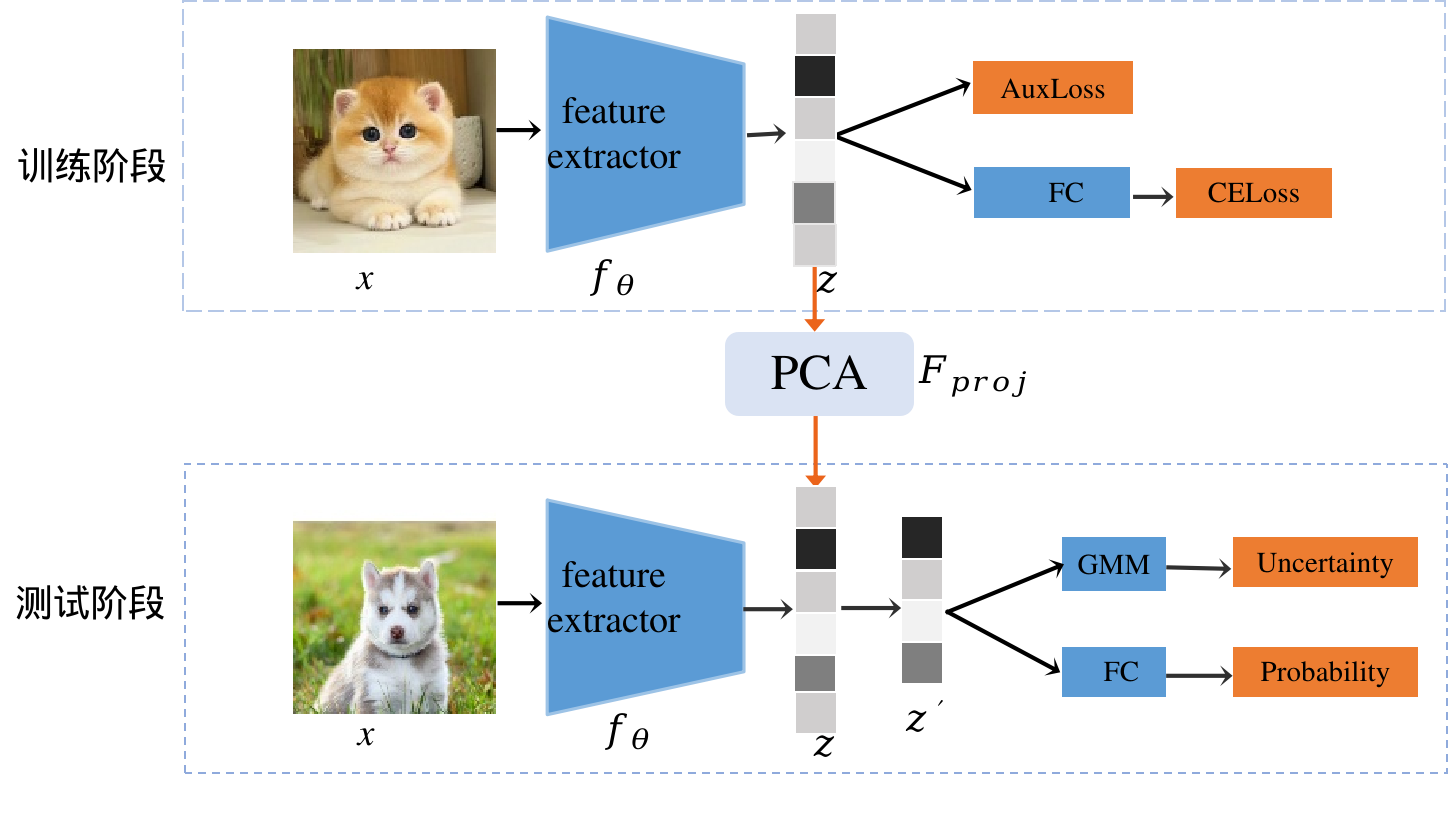
\includegraphics[width=1.\linewidth]{assets/structure3.png}
    \caption{基于高维特征概率密度建模的模型不确定性}
    \label{tag:模型结构图3}
\end{figure}


PCA(Principal Component Analysis,主成分分析)是一种常见的降维技术,用于将高维数据转换为低维数据,同时尽可能保留数据的主要特征信息。PCA通过找到数据中方差最大的方向,将数据投影到这些方向上,从而达到降维的目的。PCA应用到高维数据上,通过减少数据的维度,可以显著降低计算复杂度。在高维数据处理中,PCA常用于减少数据维度,去除冗余信息,使得后续的机器学习模型更加高效。通过降维,PCA可以去除一些噪声和无关的特征,帮助减轻过拟合问题,提高模型的泛化能力。 PCA算法主要步骤如下\cite{jolliffe1986principal}:
\begin{figure}[h]
    \centering
    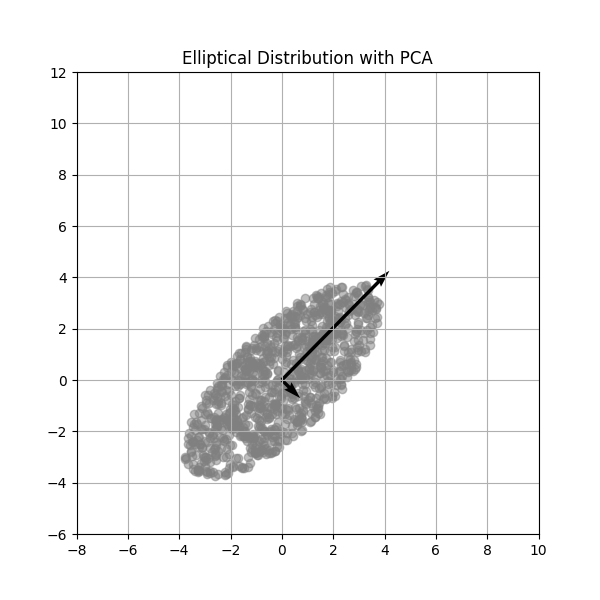
\includegraphics[width=1.\linewidth]{assets/pca.png}
    \caption{PCA原理}
    \label{tag:pca}
\end{figure}

 (1) 数据中心化:首先,对原始数据进行中心化处理,即将每个特征减去该特征的均值,使数据的均值为零

 (2) 计算数据的协方差矩阵,它描述了各个特征之间的关系和方差。对于一个 \(n \times m\) 的数据矩阵 \(\mathbf{X}\),其协方差矩阵为:$\Sigma = \frac{1}{n-1} \mathbf{X}^T \mathbf{X}$


(3) 计算特征值和特征向量
通过对协方差矩阵 \(\Sigma\) 进行特征值分解,得到其特征值和特征向量。特征向量代表了数据中变化的方向,特征值表示该方向上的方差大小。计算得到的特征向量就是主成分的方向。


(4) 选择主成分,构成转换矩阵
选择特征值最大的几个特征向量作为主成分,这些主成分保留了数据中最大的方差。选择的特征向量数量决定了降维后的维度。通过将原始数据投影到选定的主成分上,得到降维后的数据。假设选取前 \(k\) 个特征向量作为主成分,则新的数据矩阵为:

\[
\mathbf{X}_{PCA} = \mathbf{X}_{centered} \cdot \mathbf{V}_k
\]
其中,\(\mathbf{V}_k\) 是由前 \(k\) 个特征向量组成的矩阵,\(\mathbf{X}_{PCA}\) 是降维后的数据矩阵。

\textbf{在训练阶段},首先完成神经网络训练,之后在训练集上使用神经网络提取训练数据的高维特征。这些特征通常来自神经网络某一层的输出,代表输入数据的高维表示。之后对提取的高维特征进行主成分分析(PCA),计算特征协方差矩阵并对其进行特征分解,获取主成分方向。根据累计方差贡献率(如 95\% 或 99\%)选择前 k 个主成分,从高维空间降维到k维。使用 PCA 转换矩阵将原始高维训练特征投影到 k 维主成分空间,得到降维后的训练特征。在降维后的特征空间中,训练高斯混合模型(GMM),估计混合成分的均值、协方差矩阵和权重参数。训练完成后,保存 PCA 转换矩阵和 GMM 模型的参数。

\textbf{在不确定性计算阶段}。对测试数据通过同一神经网络提取高维特征,保证特征分布与训练阶段一致。使用训练阶段保存的 PCA 转换矩阵,将测试数据的高维特征投影到k 维主成分空间。注意:在此阶段,不需要计算 PCA 转换矩阵,而是必须使用训练阶段的转换矩阵以确保一致性。将降维后的测试特征输入到训练好的 GMM 模型中,计算每个数据点属于各个高斯分布成分的概率,同时直接输出分类结果(如最大后验概率对应的类别)。

总结一下,这部分分为训练阶段和不确定性计算阶段。训练阶段完成从高维特征提取、PCA建模到GMM参数估计的一系列操作,目的是学习特征空间的低维表示及其概率分布。不确定性计算阶段应用训练阶段学习到的 PCA 转换和 GMM 模型,对测试数据进行降维和分类推断。这种分阶段的操作流程能够保证训练和测试时的特征空间一致性,并大幅减少高维特征带来的计算复杂度。



多元高斯分布的概率密度函数为:

\[
p(\mathbf{z} \mid \boldsymbol{\mu_c}, \boldsymbol{\Sigma_c}) = \frac{1}{(2\pi)^{\frac{D}{2}} \left| \boldsymbol{\Sigma_c} \right|^{\frac{1}{2}}} \exp \left( -\frac{1}{2} (\mathbf{z} - \boldsymbol{\mu_c})^T \boldsymbol{\Sigma_c}^{-1} (\mathbf{z} - \boldsymbol{\mu_c}) \right)
\]
在高斯混合模型(GMM)中,假设已经完成了训练,因此均值向量和协方差矩阵已经预先计算好。假设特征向量的维度为 \( M \),对于每个类别 \( k \),计算一个特征向量的概率密度时,首先需要计算差 \( (\mathbf{z} - \mu_k) \),其时间复杂度为 \( O(M) \)。然后计算矩阵乘法 \( \Sigma_k^{-1} (\mathbf{z} - \mu_k) \),这一步的时间复杂度为 \( O(M^2) \),接着进行标量计算 \( (\mathbf{z} - \mu_k)^T \Sigma_k^{-1} (\mathbf{z} - \mu_k) \),其时间复杂度为 \( O(M) \)。此外,协方差矩阵的行列式和平方根计算已被忽略。由于这些步骤需要对每个特征向量进行计算,因此降维前的总时间复杂度为 \( O(M^2) \)。

当特征维度通过主成分分析(PCA)降到 \( N \) 维时,首先对原始特征向量进行降维。假设降维矩阵 \( P \) 已经预先计算好,降维操作的时间复杂度为 \( O(M \cdot N) \)。然后,对于降维后的 \( N \)-维特征向量,首先计算差 \( (\mathbf{z'} - \mu_k) \),其时间复杂度为 \( O(N) \),接着计算矩阵乘法 \( \Sigma_k^{-1} (\mathbf{z'} - \mu_k) \),这一步的时间复杂度为 \( O(N^2) \),最后进行标量计算 \( (\mathbf{z'} - \mu_k)^T \Sigma_k^{-1} (\mathbf{z'} - \mu_k) \),其时间复杂度为 \( O(N) \)。因此,降维后的时间复杂度为 \( O(M \cdot N + N^2) \),其中 \( O(M \cdot N) \) 是降维操作的复杂度,\( O(N^2) \) 是 GMM 计算的复杂度。

在空间复杂度方面,降维前每个类别的均值向量 \( \mu_k \) 需要 \( O(M) \) 空间,协方差矩阵 \( \Sigma_k \) 需要 \( O(M^2) \) 空间。因此,对于 \( K \) 个类别,存储所有均值向量和协方差矩阵的总空间复杂度为 \( O(K \cdot M^2) \)。特征向量 \( \mathbf{x} \) 需要 \( O(M) \) 空间。降维后的均值向量 \( \mu_k \) 需要 \( O(N) \) 空间,协方差矩阵 \( \Sigma_k \) 需要 \( O(N^2) \) 空间。因此,对于 \( K \) 个类别,存储所有均值向量和协方差矩阵的空间复杂度为 \( O(K \cdot N^2) \),降维后的特征向量 \( \mathbf{z'} \) 需要 \( O(N) \) 空间,降维矩阵 \( P \) 需要 \( O(M \cdot N) \) 空间。综上,降维后的总空间复杂度为 \( O(K \cdot N^2 + M \cdot N) \),通常由于 \( N < M \),降维后空间复杂度显著低于降维前的空间复杂度。




基于辅助损失函数联合训练并使用PCA降维加速的改进算法原理见\ref{alg:2}。


\begin{algorithm}[h]
	\caption{基于输入扰动的概率密度建模的模型不确定性算法}
	\label{alg:2}
	
	\begin{algorithmic}[1]
		\Require 训练集: $(X,Y)$ 
		\Require 高维特征提取网络: $f_{\theta}:x \rightarrow \mathbf{R}^d $ 
		\Require GMM模型: $q(z) = \max_{c}q(z|y=c)$
		
		\\
		\Procedure {1.训练阶段}{}
            \State 初始化类中心$C_i$
		\State 使用$CELoss+\lambda*AuxLoss$,在训练数据集数据集上训练网络$f_{\theta}$


		\EndProcedure
            \\
        
		\Procedure {2.PCA训练和GMM建模}{}
		\State 在训练集上抽取高维特征,并训练PCA模型$F_{proj}$
            \For {属于类别c的样本}
		\State $\mu_{c}=F_{proj}(\frac{1}{|x_c|}f_{\theta}(x_c))$
		\State $\Sigma_c = \frac{1}{|x_c|-1}(F_{proj}(f_{\theta}(x_c))-\mu_c)(F_{proj}(f_{\theta}(x_c))-      \mu_c)^T$
		\State q(y=c)=$\frac{|X_C|}{|X|}$
            \EndFor
		\EndProcedure 
            \\

        
		\Procedure {3.模型不确定性计算}{}
		\State $z=F_{proj}(f_{\theta}(x))$
		\State 计算模型不确定性 $Uncertainty(x) = \log \max_{c}q(z|y=c)$,其中$q(z|y=c)\sim N(\mu_c,\Sigma_c)$
		\EndProcedure 
	\end{algorithmic}
\end{algorithm}


\section{实验结果与分析}
为了评估本文所提出的基于输入扰动的改进对模型不确定性建模的提升,本节分别在OOD检测任务上,误分类样本识别等任务上进行了评估。本节的实验内容主要是在CIFAR-10,CIFAR-100,SVHN,MNIST,LSUN等数据集和VGG,ResNet,VIT等模型进行的。为了评估使用辅助损失函数联合训练对模型不确定建模效果的影响,本文评估单独使用交叉熵损失函数(CELoss)和辅助损失函数(AuxLoss)+交叉熵损失函数(CELoss)联合训练两种不同的训练策略得到的模型,在模型训练时,有关批次,批大小,优化器,初始学习率等超参数设置见下表格\ref{tab:模型训练2},在训练的时候针对网络权重参数和辅助损失函数里面的类中心参数,分别使用优化器1和优化器2。
\begin{table}[htbp]
	\captionsetup{font=small, justification=centering}
	\centering
	\resizebox{\linewidth}{!}{
	\begin{tabular}{c c c c c c c c c c c}
	\hline
	模型结构 & 数据集 & 批次 & 批大小 & $\lambda$ & 优化器1 & 优化器2 & 优化器1学习率 & 优化器2学习率 & 动量 & 权重衰减 \\
	\hline
	VGG16 & CIFAR10 & 300 & 512 & 20 &SGD & SGD & 0.1  & 0.5 & 0.9 & 0.0005 \\
        ResNet50 & CIFAR10 & 300 & 512 & 20 &  SGD & SGD  & 0.5  & 0.1 & 0.9 & 0.0005 \\
        VIT & CIFAR10 & 300 & 512 &  20 &  SGD & SGD & 0.01  & 0.5 & 0.9 & 0.0005 \\
	\hline
	\end{tabular}
	}
	\caption{
	模型训练超参数设置
	}
        \label{tab:模型训练2}
\end{table}


\subsection{OOD检测任务上评估}

以上通过可视化特征空间,验证了所提出的新的辅助损失函数和交叉熵损失函数联合训练,能够提升特征空间上不同类别样本的类内紧密性和类间可分性。为了验证联合训练基于高维特征概率密度建模不确定性的影响,本节在OOD检测任务上评估使用辅助损失函数联合训练对模型不确定建模效果的影响,本节选择CIFAR10数据集的训练集,使用交叉熵损失函数(CELoss)单独训练VGG/ResNet50/VIT等不同模型,然后再使用辅助损失函数(AuxLoss)和交叉熵损失函数(CELoss)联合训练的策略训练VGG/ResNet50/VIT等不同模型。使用CIFAR10数据集的测试集作为分布内样本(inD样本),SVHN、CIFAR100、LSUN、MNIST等数据集作为分布外样本(OOD样本),构建OOD检测任务,评估两种不同的训练策略对模型不确定性的建模效果,实验结果如表\ref{OOD}。


\begin{table}[h]
\captionsetup{font=small, justification=centering}
\centering
\renewcommand{\arraystretch}{1.2}
\setlength{\tabcolsep}{8pt}
\begin{tabular}{c c c c c}
\hline
\textbf{训练策略} & \textbf{OOD Dataset} & \textbf{VGG} & \textbf{ResNet} & \textbf{ViT} \\ 
\hline
\multirow{4}{*}{CE Loss} 
& SVHN & 0.9190/0.9423 & 0.9095/0.9367 & 0.9767/0.9835 \\ 
& LSUN & 0.9086/0.9167 & 0.9205/0.9393 & 0.9858/0.9886 \\ 
& CIFAR100 & 0.8832/0.8976 & 0.8898/0.9014 & 0.9476/0.9534 \\ 
& MNIST & 0.9195/0.9399 & 0.8991/0.9276 & 0.9606/0.9687 \\ 
\hline
\multirow{4}{*}{联合训练} 
& SVHN & \textbf{0.9293/0.9506} & \textbf{0.9445/0.9580} & \textbf{0.9835/0.9872} \\ 
& LSUN & \textbf{0.9164/0.9230} & \textbf{0.9313/0.9455} & \textbf{0.9888/0.9906} \\ 
& CIFAR100 & \textbf{0.8927/0.9059} & \textbf{0.9025/0.9140} & \textbf{0.9566/0.9588} \\ 
& MNIST & \textbf{0.9322/0.9529} & \textbf{0.9470/0.9588} & \textbf{0.9854/0.9874} \\ 
\hline
\end{tabular}
\caption{OOD检测任务上评估,合并后的实验结果,显示不同训练策略和模型在多个 OOD 数据集上的表现。}
\label{OOD}
\end{table}


从表格\ref{OOD}结果可以看出,加入辅助损失函数的联合训练策略在各模型(VGG、ResNet、ViT)和多个数据集(SVHN、LSUN、CIFAR100、MNIST)的OOD检测任务上均显著提升了AUROC/AUPRC指标,这表明联合训练策略的引入有效增强了模型在 OOD 数据集上的检测能力,表现为更高的 AUROC 和 AUPR 分数。使用新提出的损失函数联合训练的策略在OOD检测任务上的效果提升,验证了在使用辅助损失函数联合训练的特征空间上进行概率分布的建模,能更好地建模神经网络的不确定性。

\subsection{误分类样本检测任务上评估}

误分类样本检测任务用于评估神经网络在预测结果上的不确定性,是通过模型能否依据不确定性值识别出自身预测错误的样本。本节在CIFAR10数据集的训练集上,使用交叉熵损失函数(CELoss)和辅助损失函数(AuxLoss)+交叉熵损失函数(CELoss)联合训练两种不同的训练策略训练VGG/ResNet50/VIT等不同模型,并在CIFAR10测试集进行误分类检测实验,实验结果如图\ref{tab:misclassified2}。

实验结果表明,加入辅助损失函数联合训练的改进方法在所有模型上均显著提升了 AUROC 和 AUPRC 指标,这表明加入辅助损失函数联合训练能够有效增强模型对误分类样本的检测能力,提高模型的不确定性建模能力。

同时本实验评估了加入辅助损失函数前后训练出的模型的校准性能,该性能由ECE指标表示,ECE指标越小说明模型校准能力越好。从表\ref{tab:misclassified}中可以看出,加入辅助损失函数联合训练的改进方法在所有模型上在ECE指标上均降低了,ECE指标越低表明模型的预测概率与实际准确率之间的匹配程度较好,即模型是校准良好的,由此得出结论:辅助损失函数联合训练的改进方法能够提高模型的校准性能。
\begin{table}[h]
    \captionsetup{font=small, justification=centering}
    \centering
    \renewcommand{\arraystretch}{1.0} % Adjust line spacing
    \resizebox{\linewidth}{!}{
    \begin{tabular}{l l c c c}
    \toprule
    Method & Model & AUROC($\uparrow$) & AUPRC($\uparrow$) & ECE($\downarrow$) \\
    \midrule
    \multirow{5}{*}{\vspace{4em} CELoss} 
    & VGG16 & 0.9274  & 0.9945 & 0.0404\\
    & ResNet50 &  0.9344 & 0.9963 & 0.0286 \\
    & VIT & 0.9481 & 0.9984 &0.0167 \\
    \midrule
    \multirow{5}{*}{\vspace{4em} 联合训练} 
    & VGG15 & \textbf{0.9343} & \textbf{0.9951} & \textbf{0.0401} \\
    & ResNet50 & \textbf{0.9450}  & \textbf{0.9969} &\textbf{0.0344}\\
    & VIT & \textbf{0.9479}  & \textbf{0.9980} &\textbf{0.0166}\\
    \bottomrule
    \end{tabular}
    }
    \caption{误分类样本检测任务,实验结果在不同的模型(VGG16、ResNet50、VIT)上做实验,对比交叉熵损失函数训练和使用辅助损失函数联合训练对模型不确定性的建模效果,报告指标是AUROC($\uparrow$) / AUPRC($\uparrow$)/ECE($\downarrow$)}
    \label{tab:misclassified2}
\end{table}


\subsection{PCA降维对模型不确定性的影响}

高维特征概率密度建模面临维度灾难、计算复杂度和过拟合风险等挑战,为解决这些问题,本文采用PCA降维技术来减少特征空间的复杂性,提升建模效果。本节实验探究PCA算法降维前后,在OOD检测任务上模型不确定性的表现,算法实现使用sklearn.decomposition.PCA,该实现中最重要的参数是n\_components,表示降维后的保留特征的维度大小。在 sklearn.decomposition.PCA 中,n\_components参数用于控制PCA算法选择的主成分数量,具体设置方式如下:

\begin{enumerate}
  \item \textbf{整数值} ($n\_components = k$):
    如果 $n\_components$ 设置为一个整数 $k$,则PCA会选择保留前 $k$ 个主成分,$k$ 需要小于或等于输入数据的特征数 。这样做会将数据降维到 $k$ 个维度。

  \item \textbf{浮点数} ($0 < n\_components < 1$):
    如果 $n\_components$ 设置为介于0和1之间的浮动值(如0.95),PCA将选择最小的主成分数,以保证这些主成分解释的数据方差比例大于该浮动值。
  \item \textbf{'mle'} :
    如果 $n\_components$ 设置为 'mle',PCA会使用Minka的MLE方法自动选择最合适的主成分数。该方法通过估计数据的协方差矩阵的最大似然估计来决定主成分的数量。


\end{enumerate}

实验中在CIAFR10数据集上训练了不同的模型(VGG16、ResNet50、VIT),PCA算法设置n\_components采用网格搜索的方法,从128到最到维度按照间隔32搜索最合适的维度。在训练数据集的特征上训练PCA模型,然后在OOD检测任务上评估加入PCA降维前后模型的不确定性建模效果。实验结果见表\ref{tab:PCA_results_CIFAR10}
\begin{table}[h]
    \captionsetup{font=small, justification=centering}
    \centering
    \renewcommand{\arraystretch}{1.0} % Adjust line spacing
    \resizebox{\linewidth}{!}{
    \begin{tabular}{l l c c c}
    \toprule
    Method & OOD Dataset & VGG16+CIFAR10 & ResNet50+CIFAR10 & VIT+CIFAR10 \\
    &  & (Accuracy=0.9405) & (Accuracy=0.9489) & (Accuracy=0.9658) \\
    \midrule
    \multirow{4}{*}{联合训练} 
    & SVHN & 0.9190 / \textbf{0.9423} & 0.9102 / 0.9374 & 0.9835 / 0.9872 \\
    & LSUN & 0.9055 / 0.9255 & 0.9365 / 0.9232 & 0.9888 / 0.9906 \\
    & CIFAR100 & 0.8838 / 0.8972 & \textbf{0.9068} / 0.8883 & 0.9566/ 0.9588 \\
    & MNIST & 0.9206 / 0.9405 & 0.9005 / 0.9305 & 0.9849 / 0.9870 \\
    \midrule
    \multirow{4}{*}{联合训练+PCA} 
    & SVHN & \textbf{0.9200} / 0.9419 & \textbf{0.9197} / \textbf{0.9413} & \textbf{0.9846} / \textbf{0.9879} \\
    & LSUN & \textbf{0.9197} / \textbf{0.9343} & \textbf{0.9365} / \textbf{0.9455} & \textbf{0.9898} / \textbf{0.9914} \\
    & CIFAR100 & \textbf{0.8910} /\textbf{ 0.9030} & 0.9031 / \textbf{0.9137} & \textbf{0.9571} / \textbf{0.9580} \\
    & MNIST & \textbf{0.9304} / \textbf{0.9465} & \textbf{0.9282} / \textbf{0.9957} & \textbf{0.9858} / \textbf{0.9879} \\
    \bottomrule
    \end{tabular}
    }
    \caption{数据集选择CIFAR10,在不同的模型(VGG16,ResNet50,VIT)上做训练,对比联合训练和联合训练+PCA降维对模型不确定性的建模效果,报告指标是AUROC($\uparrow$) / AUPRC($\uparrow$)}
    \label{tab:PCA_results_CIFAR10}
\end{table}

加入PCA降维后,在一些模型和数据集上的AUROC和AUPRC指标显著提高。这表明,PCA能够帮助降低高维数据的噪声,在低维空间上更容易建模分布,减弱高维空间上存在的稀疏性和维度灾难等问题,进而提高OOD检测的性能。对于VGG16这样相对简单的模型,PCA的提升效果较小,因为VGG16本身提取的高维特征512维相对较低。分析降维后有些数据集上OOD检测能力提升,可能的原因时模型能够更加聚焦于关键特征,减少冗余信息的干扰,从而提高不确定性建模和OOD检测的效果。



\subsubsection{PCA与维度的分析}

PCA降维中维度大小对结果有很大的影响,本节实验还探讨了模型不确定性建模效果与PCA降维特征维度的关系。实验中在CIFAR10数据集上训练ResNet50模型,对于训练数据抽取的特征使用PCA降维,设置n\_components参数为整数并使用网格搜索遍历[256,512,1024]等不同维度,统计降维前后在OOD检测任务上的时间、存储、以及AUROC/AUPRC指标,实验结果见\ref{fig:PCA-dimension}

\begin{figure}[h]
    \captionsetup{font=small, justification=centering}
    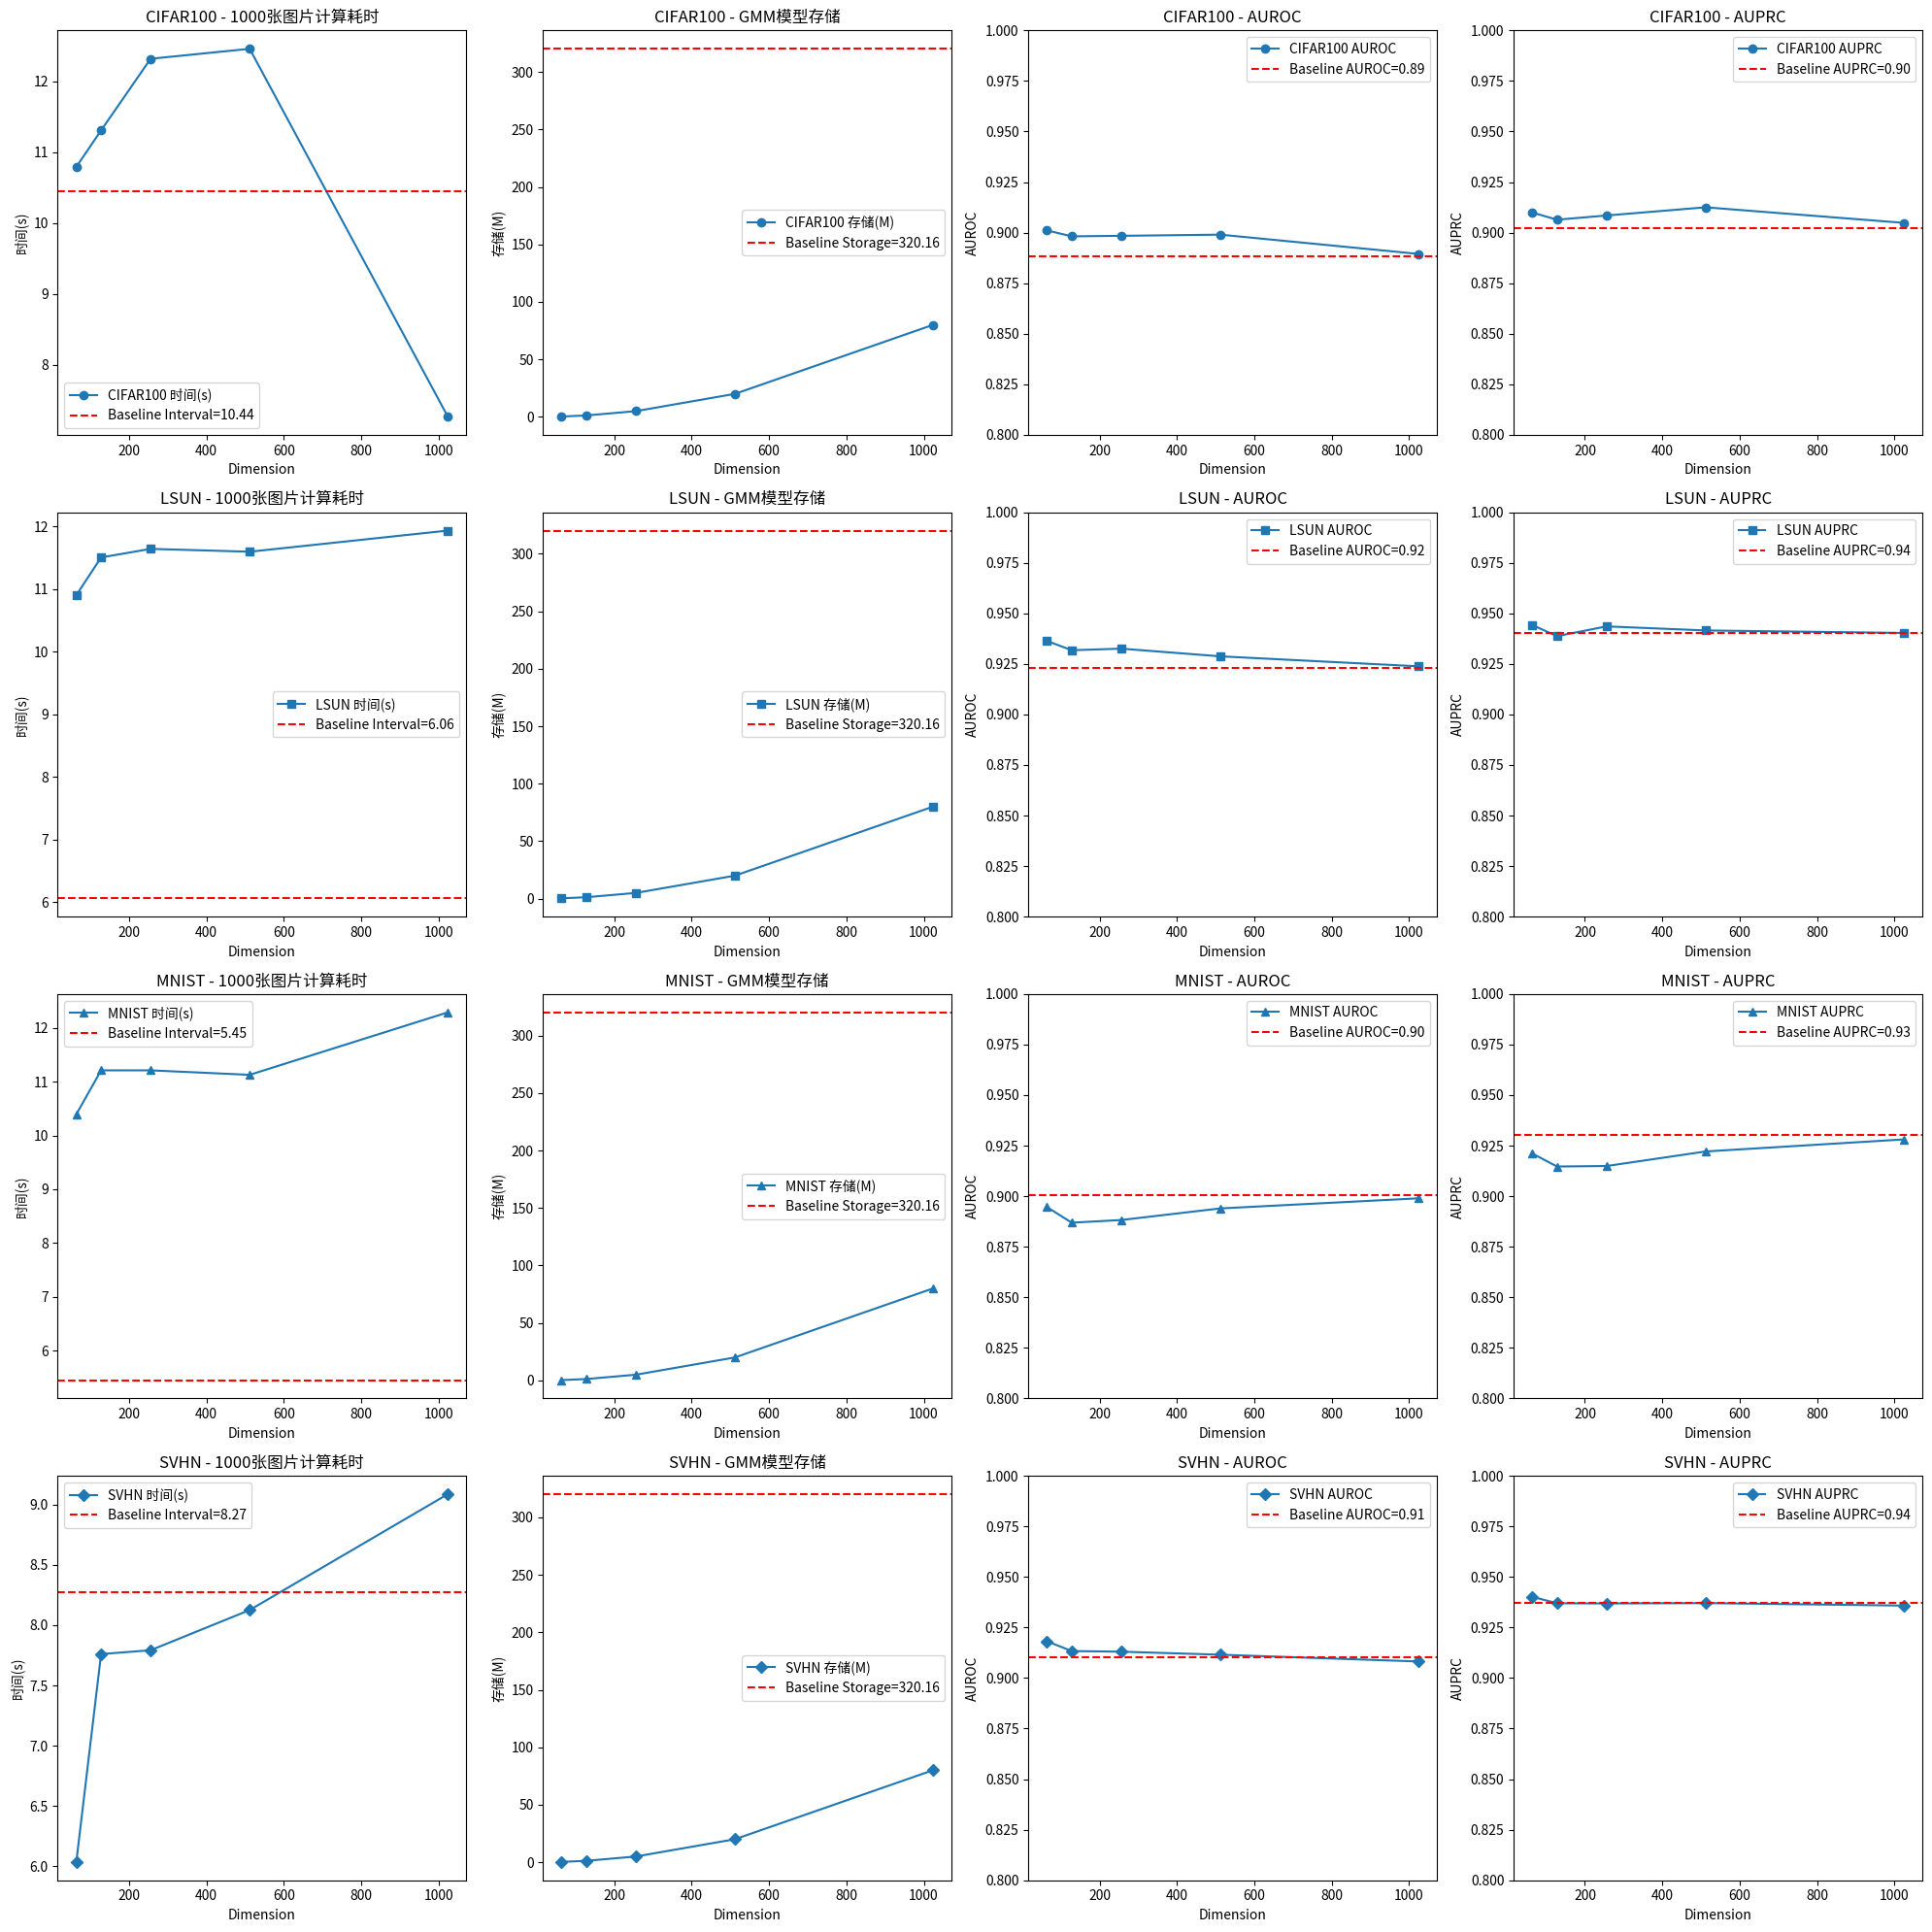
\includegraphics[width=1.\linewidth]{assets/pca_plots_dimension.png}
    \caption{PCA维度的分析,红色基线是未降维时的结果,蓝色线是在不同维度下的不同指标随降维维度的变化趋势}
    \label{fig:PCA-dimension}
\end{figure}

从图\ref{fig:PCA-dimension}中可以看出,实验在 CIFAR-100、LSUN、MNIST 和 SVHN 四个数据集上分析了 PCA 降维在不同维度(256 至 1024 维)下对计算时间、存储需求以及对模型不确定性建模效果(通过OOD检测任务上的AUROC 和 AUPRC指标反映)的影响。结果表明,计算时间随着维度的增加显著增长,高维度情况下的计算开销尤为明显,同时整体上看降维后的计算耗时都高于基线,这与上面降维后时间复杂度降低的理论分析相矛盾,这是因为在实验中PCA算法是使用sklearn中的实现,计算是在CPU上进行的,降维后的计算时间一部分在CPU计算,一部分在GPU上计算,相比降维前全都在GPU上运算,可能会出现降维后计算时间反而变大。高斯混合模型的参数均值和协方差矩阵的存储需求也随着维度增长,且在所有的维度上,降维后存储开销显著低于基线模型,展现出良好的存储效率,且存储随着维度的变化接近指数增长,与前文的理论分析一致。与此同时,AUROC 和 AUPRC 两项性能指标在各数据集上的没有因为降维大幅度减少,即使在较低维度(如 256 维)情况下,对不确定性的建模效果几乎未受到影响,说明 PCA 能够在显著降低数据规模的同时很好地保留数据的关键信息,在某些数据集上AUROC/AUPRC降维后甚至会升高,这可能是因为在降维后减弱了高维情况下可能出现的维度灾难。

综合以上分析为了降低计算开销,建议在实际应用中结合计算资源限制选择较低的降维维度(如 256-512 维)。综合存储需求、计算时间和性能指标的变化,选择 256-512 维 是较为合理的范围,可以在存储和性能之间取得最佳平衡。

\subsection{消融实验}
在联合训练的基础上,结合第三章提出的基于输入扰动的改进,在OOD检测任务上评估。实验首先在CIFAR10数据集上进行VGG16/ResNet50/VIT等模型的训练,训练完成后在SVHN/LSUN/CIFAR100/MNIST等数据集上进行OOD检测任务的评估。实验结果见表\ref{tab:combined_3_4}

\begin{table}[h]
	\captionsetup{font=small, justification=centering}
	\centering
	\renewcommand{\arraystretch}{1.0} % Adjust line spacing
	\resizebox{\linewidth}{!}{
		\begin{tabular}{l l c c c}
			\toprule
			Method & OOD Dataset & VGG16+CIFAR10 & ResNet50+CIFAR10 & VIT+CIFAR10 \\
			&  & (Accuracy=0.9405) & (Accuracy=0.9489) & (Accuracy=0.9600) \\
			\midrule
			\multirow{4}{*}{CE} 
                & SVHN & 0.9190/0.9423 & 0.9095/0.9367 & 0.9767/0.9835 \\ 
                & LSUN & 0.9086/0.9167 & 0.9205/0.9393 & 0.9858/0.9886 \\ 
                & CIFAR100 & 0.8832/0.8976 & 0.8898/0.9014 & 0.9476/0.9534 \\ 
                & MNIST & 0.9195/0.9399 & 0.8991/0.9276 & 0.9606/0.9687 \\ 
			\midrule
			\multirow{4}{*}{联合训练} 
            & SVHN & 0.9293/0.9506 & 0.9445/0.9580 & \textbf{0.9835/0.9872} \\ 
            & LSUN & 0.9164/0.9230 & 0.9313/0.9455 & \textbf{0.9888/0.9906} \\ 
            & CIFAR100 & 0.8927/0.9059 & 0.9025/0.9140 & \textbf{0.9566/0.9588} \\ 
            & MNIST & 0.9322/0.9529 & 0.9470/0.9588 & \textbf{0.9854/0.9874} \\ 
			\midrule
			\multirow{4}{*}{联合训练+输入扰动} 
			& SVHN & \textbf{0.9316/0.9511 }& \textbf{0.9835/0.9869} & 0.9828/0.9893 \\
			& LSUN & \textbf{0.9494/0.9633} &\textbf{ 0.9771/0.9816} & 0.9788/0.9740 \\
			& CIFAR100 & \textbf{0.8985/0.9109 }& 0.\textbf{9271/0.9472} & 0.9563/\textbf{0.9695} \\
			& MNIST & \textbf{0.9637/0.9766} &\textbf{ 0.9847/0.9887} & \textbf{0.9984/0.9926} \\
			\bottomrule
		\end{tabular}
	}
	\caption{在CIFAR10数据集上训练VGG/ResNet50/VIT等模型,选取SVHN、CIFAR100、MNIST、LSUN等数据集作OOD数据集,在OOD检测任务上做实验对比CrossEntropy训练、CrossEntropy+AuxLoss联合训练、联合训练+输入扰动对模型不确定性的建模效果,报告指标是AUROC($\uparrow$) / AUPRC($\uparrow$),越高越好}
	\label{tab:combined_3_4}
\end{table}



表格\ref{tab:combined_3_4}中的实验结果展示了在不同模型(VGG16、ResNet50、VIT)上对四个OOD数据集(SVHN、LSUN、CIFAR100、MNIST)的OOD检测性能的影响,评估了三种方法(CrossEntropy、CrossEntropy+AuxLoss联合训练、联合训练+输入扰动)对模型不确定性的建模效果。从OOD检测结果来看,加入辅助损失函数联合训练结合输入扰动的方法在相比于另外两种单纯使用交叉熵损失训练和仅联合训练的方法,在所有模型和数据集上均显著提升了检测性能,这表明辅助损失函数联合训练的方法增强了模型对模型不确定性的捕捉能力,而输入扰动进一步提高了对不确定性的建模能力。加入AuxLoss的联合训练策略在增强模型对类间分布的区分能力方面表现出显著优势,而引入输入扰动进一步提高了模型在复杂分布下不确定性建模的鲁棒性和泛化能力。。

\section{本章小结}
本章提出的核心方法是通过优化特征空间结构来提升不确定性建模的效果。神经网络的分类性能和不确定性量化能力直接依赖于特征空间的质量。理想的特征空间应具备高类内样本紧密性和较大类间可分性,这有助于模型更好地区分不同类别,提升其稳定性和鲁棒性。然而,在实际应用中,神经网络通常难以同时优化这两个方面,导致特征空间分布混乱,进而影响模型表现。为解决这一问题,被提出作为提升特征空间质量的重要方法。度量学习通过优化损失函数,使得同一类别的样本尽可能紧密,而不同类别的样本保持较大间距,从而改善模型的分类性能。传统的CenterLoss通过增强类内紧密性来优化特征空间,但未充分考虑类别间的分隔性,可能导致类别重叠或混淆,特别是在高维数据中。这一问题直接影响模型的分类精度和不确定性量化能力。

为此,本章提出了一种新型损失函数——AuxLoss。AuxLoss在传统CenterLoss的基础上引入了类别中心间距的约束,不仅加强了类内样本的聚集效果,还优化了类间的分隔性。实验结果表明,结合AuxLoss的模型在多个数据集上取得了优异的表现,尤其在MNIST和CIFAR-10等数据集上,模型在分类精度和特征空间分布上均有显著提升。通过t-SNE可视化,优化后的模型在低维空间中展现出更加清晰的类别边界,类别间的分隔更加明显,进一步提升了模型的分类稳定性和鲁棒性。

在定量评估方面,结合AuxLoss的模型在特征空间质量方面表现突出。使用Davies-Bouldin指数和Fisher比率等指标进行评估时,结果显示AuxLoss显著提高了类内样本的聚集性和类间样本的可分性,从而增强了模型对不确定性的量化能力,使得模型在复杂任务中更加稳定和可靠。

此外,本章还探讨了如何结合PCA降维与高斯混合模型来应对高维数据建模中的计算复杂性问题。PCA能够有效降低数据的维度,同时保留主要方差,减少计算开销和存储空间。实验表明,结合PCA降维和GMM的模型在高维数据处理上取得了优异效果,特别是在MNIST和CIFAR-10等复杂数据集上,不仅提升了模型性能,还有效降低了高斯混合模型的存储消耗。

总体而言,本章提出的特征空间优化方法,通过结合度量学习、AuxLoss损失函数以及PCA-GMM降维,显著提高了神经网络的分类精度和不确定性量化能力。这些研究不仅推动了神经网络不确定性建模的理论发展,也为实际应用中的异常检测、风险评估等任务提供了有力支持。未来的研究将着重于进一步优化特征空间结构,并探索更高效的不确定性量化方法。